\documentclass[tikz,border=2pt]{standalone}
\usetikzlibrary{arrows.meta,calc}
\begin{document}
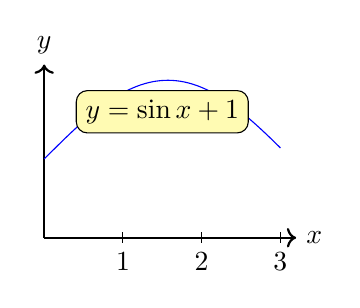
\begin{tikzpicture}
  \draw[->,thick] (0,0) -- (3.2,0) node[right] {$x$};
  \draw[->,thick] (0,0) -- (0,2.2) node[above] {$y$};
  \draw[blue, domain=0:3, samples=60] plot (\x, {sin(\x r)+1});
  \node[fill=yellow!30,draw,rounded corners] at ($(1.5,1.6)$) {$y=\sin x + 1$};
  \foreach \i in {1,2,3} \draw (\i,2pt) -- (\i,-2pt) node[below] {\i};
\end{tikzpicture}
\end{document}
